%
% File coling2016.tex
%
% Contact: mutiyama@nict.go.jp
%%
%% Based on the style files for COLING-2014, which were, in turn,
%% Based on the style files for ACL-2014, which were, in turn,
%% Based on the style files for ACL-2013, which were, in turn,
%% Based on the style files for ACL-2012, which were, in turn,
%% based on the style files for ACL-2011, which were, in turn, 
%% based on the style files for ACL-2010, which were, in turn, 
%% based on the style files for ACL-IJCNLP-2009, which were, in turn,
%% based on the style files for EACL-2009 and IJCNLP-2008...

%% Based on the style files for EACL 2006 by 
%%e.agirre@ehu.es or Sergi.Balari@uab.es
%% and that of ACL 08 by Joakim Nivre and Noah Smith

\documentclass[11pt]{article}
\usepackage{coling2016}
\usepackage{times}
\usepackage{url}
\usepackage{latexsym}
\usepackage{graphicx}
\usepackage{amsmath}


%\setlength\titlebox{5cm}

% You can expand the titlebox if you need extra space
% to show all the authors. Please do not make the titlebox
% smaller than 5cm (the original size); we will check this
% in the camera-ready version and ask you to change it back.


\title{Optimization of the Modeling Approach for Predicting the Tolerance Level of Religious Discourse}

\author{Nicolas Venuti \\
  Data Science Institute \\
  University of Virginia \\
  Charlottesville, VA USA \\
  {nmv7de@virginia.edu} \\\And
  Hope McIntyre \\
  Data Science Institute \\
  University of Virginia \\
  Charlottesville, VA USA \\
  {hm7zg@virginia.edu}\\\And
  Donald E. Brown \\
  Data Science Institute \\
  University of Virginia \\
  Charlottesville, VA USA \\
  {brown@virginia.edu} \\}

\date{}

\begin{document}
\maketitle
\begin{abstract}
Religious violence is one of the biggest and most complicated problems facing the world today. The number of incidents has been increasing in recent years and, unfortunately, scalable and accurate systems to predict which groups are likely to engage in such actions are not keeping pace. Additionally, this problem is compounded by lingual and cultural differences, which limit the effectiveness of understanding how tolerant or intolerant a group is without bias. To circumvent this challenge, recent studies indicate promise in the analysis of the performative character of discourse (how words are used) to estimate the tolerance level, rather than using the semantic or emotive character of text (what the words mean or imply). Using expert estimates of linguistic flexibility, a representation of the performative character of text, and thus also predictive of a text’s tolerance level, this paper describes (a) new approaches to automating the quantification of the performative character of words and (b) the predictive efficacy of these approaches versus traditional semantic indicators of tolerance or intolerance. To implement the pipeline, a judgment identifier was developed along with multiple semantic density algorithms to extract the frequency of judgments and flexibility of keyword contexts, respectively. Test results show that text mining algorithms can accurately estimate the language flexibility of religious discourse. These results provide evidence that the performative characteristics of language better predict tolerance level than the semantic characteristics of language.


\end{abstract}

\section{Introduction}\label{Intro}

\blfootnote{
    %
    % 
    %
    \hspace{-0.65cm}  
    This work is licenced under a Creative Commons 
     Attribution 4.0 International License.
     License details:
     \url{http://creativecommons.org/licenses/by/4.0/}
    %
    
}

Religious violence has long been one of the most destructive and divisive acts impacting society and, unfortunately, the number of casualties associated with these acts has been rising in recent years. For example, in 2014 alone, 12,737 deaths could be attributed to the operations of just two separate radical terrorist groups: Boko Haram with 6,664 deaths, and the Islamic State of Iraq and The Levant (ISIL), with 6,073 deaths ~\cite{Searcey2015}. Unfortunately, scalable and accurate systems to predict such actions are not keeping pace with the evolution of these groups ~\cite{Yang2010}. In an effort to combat these actions, the University of Virginia Global Covenant of Religions Ethnolinguistics Research Team (GCR-ERT) has been exploring methods of diagnosing tendencies to violence through linguistic analysis.

While analyses of groups is typically done by examining the literal or emotive attributes of keywords distributed by the semantic characteristics of these words, the GCR-ERT found that it was insufficient to utilize solely semantic analysis as a method to estimate the level of tolerance displayed within religious discourse. Through their research, the GCR-ERT has found that the performative character of discourse, the capacity for language to encapsulate an action or identity, is correlated to the level of intolerance within that discourse. To quantify this performative character of discourse, the GCR-ERT have developed a 1 - 9 language rigidity scale which is used to classify texts as either rigid (scored a 1) or elastic (scored a 9). These rankings were assigned manually by analyzing a wide array of characteristics within religious discourse. To assist the GCR-ERT in their efforts, the University of Virginia Computational Linguistics Data Science (CLDS) team previously developed a text mining pipeline to (a) conduct preliminary research on automating the quantification of the performative character of words and (b) test the predictive efficacy of these implementations versus traditional semantic indicators of tolerance or intolerance. Through the manual process, the GCR-ERT discovered that certain characteristics of discourse, such as the frequency of judgments and the rigidity of keyword contexts, can be used to assist in their quantification. Through this analysis the CLDS were able to show that automated systems can be developed to model the language flexibility of religious discourse, and that performative characteristics of language yield better prediction signals than semantic characteristics of language.

To build upon this previous work, the CLDS reviewed the efficacy of hyperparameter optimization on the most predictive models from the previous study; namely random forests and SVM using features derived from sentiment analysis, context vector similarity, network quantification and judgement density. In order to perform this analysis multiple grid searches were conducted over a variety of signal parameters to determine the optimal model and feature engineering configuration. Furthermore, additional data was added to the analysis to assist in eradicating the class imbalance found in the previous analysis.

\section{Related Work}\label{relatedwork}

Because religious violence is a far-reaching and complex problem, many resources, such as intelligence analysts and NGOs, are dedicated to studying the actions and words of groups identified as high-risk. Most of these approaches, however, are not quantitative in nature. They are instead supported by the expertise of trained individuals familiar with the group’s historic behavior and rhetoric instead of scientific techniques. Research on predicting religious violence using quantitative approaches is limited. One study conducted by a research group at New Mexico State University used Latent Semantic Analysis to track temporal shifts in language usage for Iranian leaders. While topical shifts were identified in this approach, few predictive capabilities were developed through this methodology ~\cite{Hacker2013}. When quantitative methodologies are used, they tend to be fixated on predicting specific incidences of violence ~\cite{Yang2010}. Given these facts, we focused our research on the literature base surrounding methods which automatically detect semantic change. 

According to \newcite{Barsalou1993}, “the conceptualization of an entity or set of entities can vary widely across individuals and occasions”. Barsalou tested this hypothesis by providing subjects with a group of nouns such as bachelor, bird and chair and asking his subjects to provide definitions for those terms. Through his experiments he found that only “44\% of the features in one subject’s definition existed in another subject’s definition” which was likely due to the beliefs and experiences individuals have in characterizing a concept \cite{Barsalou1993}. These results assist in confirming the GRC-ERT’s hypothesis that shifts in definitions correlate with the representational flexibility of a concept.

Studying semantic change through computation is a budding research area as the development of advanced computational resources and large data repositories has made the study more feasible. Results have established the feasibility of extracting word meaning from usage patterns ~\cite{Bullinaria2007,Lin1998}. While explicit word meanings were not directly studied, a mid-stage between ‘usage patterns’ and ‘word meaning’ is a mapping to a space which notes how words tend to be used, which are potential quantitative measures for the performative characteristics of words.

\newcite{Sagi2009} attempted to detect semantic change by measuring the diversity of contexts in which a word was used. They measured “broadening” (a word meaning becoming less restricted), “narrowing” (a word becoming more specific), and “pejoration” (a meaning becoming more negative). The notion of “diversity of contexts” directly correlates with the concept of performative characteristics of word. Given this, we decided to directly test the efficacy of this method. 

\newcite{Boussidan2011} used a graph built from subsetted co-occurrence tables to create a map of lexical usages of words. Finding the cliques in this graph leads to words grouped on a semantic plane where “drunk” and “stagger” are connected despite different definitions because they are used in very similar contexts. While the work has interesting results, the requirement of computing cliques is computationally complex, limiting the scalability and accessibility of this method.

\newcite{Cook2010} attempted to detect “amelioration” (a word losing a negative meaning) and “pejoration” through a similar method. This was done by computing the average pointwise mutual similarity between a word and a set of assumed pejorative or positive words [12]. Unfortunately, this method doesn’t create an intermediate space which could be connected to performative characteristics.

Work done by \newcite{venuti2016} validated the efficacy of characteristics of language as a signal to predict the tolerance level of religious discourse. To reach this conclusion, the CLDS developed a judgment identifier along with multiple semantic density algorithms to replicate the frequency of judgments and rigidity of keyword contexts. The CLDS tested the effectiveness of these implementations against two traditional semantic indicators as baselines: a topic model and sentiment analysis. Using three classification models (SVM, neural networks, and random forest), the CLDS compared the traditional semantic signals against the performative signals to predict linguistic flexibility as determined by subject matter experts. Through this analysis the CLDS were able to show that automated systems can be developed to assist in modeling the language flexibility of religious discourse, and that performative characteristics of language yield better prediction signals than semantic characteristics of language. Limitations of this work included minimal hyperparameter exploration and optimization and a class imbalance in the data set. 

\newcite{Bullinaria2012} evaluated the impact of the application of stop-lists, word stemming, and singular value decomposition (SVD) on the performance of word-word co-occurrence statistics by comparing performance with several generic semantic tasks. They determined that neither word stop-lists nor word stemming significantly impacted performance, minimal context window size gave the best performance, and dimensionality reduction through SVD can improve performance.  

\section{Data}\label{data}

The CLDS team obtained the data used to perform this analysis from online repositories that contained texts from different religious groups with a wide variety of affiliations and language rigidities, as described in Table \ref{table:data}. We collected these texts from their respective online repositories using BeautifulSoup in Python and converted to .txt files prior to the pre-processing stage ~\cite{Richardson2015}. Following this step, the GCR-ERT manually reviewed and annotated the overall document sets with a language flexibility ranking to serve as ground truth.

\begin{table}[ht]
\caption{Data Sources}
\begin{center}
\begin{tabular}{lccc}
 \\  \hline
Group & Rank & Affiliation & Number of Doc.  \\ \hline
Westboro Baptist Church 		& 1 & Baptist		& 419 \\
Faithful Word Baptist Church	& 2 & Baptist		& 228 \\
Nouman Ali Khan			& 3 & Sunni Muslim	& 88 \\
Dorothy Day				& 4 & Catholic		& 774 \\
John Piper				& 4 & Baptist		& 579 \\
Steve Shepherd			& 4 & Christian		& 728 \\
Rabbinic texts				& 6 & Jewish		& 166 \\
Unitarian texts				& 7 & Unitarian		& 276 \\ 
Meher Baba				& 8 & Spiritualist	& 265 \\	

\end{tabular}
\end{center}
\label{table:data}
\end{table}

To balance the requirements for increased observations for modeling and the text size requirements for the semantic density algorithms, we randomly placed the documents into bins of 10 for each group. If any individual bin was smaller than half the targeted bin size (i.e. 5 documents), we discarded it so as to not introduce significant sample size disparities. For each group the bins were split into a training set containing 70\% of the bins and a testing set containing the remaining 30\%. 

We normalized and cleaned all the documents prior to signal development to ensure data continuity between each algorithm. We extracted the raw text for each bin, tokenized,  and normalized the text by removing punctuation, converting to lowercase, and converting all numbers to a single symbol. The tokens were stemmed, but stopwords were not removed. We used these tokens as the inputs for all signals with the exception of the judgement algorithm.

To identify keywords for the analysis, we applied the Maxent POS Tagger from the python nltk package  to the corpus in order to develop the list of keywords which were used as input to the context vector and network algorithms \cite{NLTK}. Word counts were generated for each unique word/POS tag combination for each bin. The top 10 most frequent adjectives and adverbs were selected for each bin and used to as the keywords. This method was proposed by the GRC-ERT based on their experience extracting keywords from religious discourse. These keywords were then fed into the context vector and network quantification analyses. 

\section{Signals}

Similar to the methods performed in the previous study, we constructed four signals as input to the model; context vector similarity, judgement fractions, document sentiment, and network quantification. Modifications were made to the judgement and sentiment algorithms in an attempt to better model the requisite features, and to provide more normalized outputs. These methods were reconstructed in python, rather than R, to provide quicker computations, and greater modeling flexibility. The algorithms for the computation of each signal as implemented in this study are described below.

\subsection{Sentiment}

We created four sentiment metrics for each group of documents: average percent positive words per document, average percent negative words per document, percent positive documents, and percent negative documents. The sentiment was calculated using a lexicon-based approach. A dictionary of approximately 6,800 positive and negative words, developed by \newcite{Liu2013}, was used. These words were stemmed as discussed in the pre-processing steps above to ensure maximal matching between the sentiment word list and the pre-processed text. Average percent positive words was calculated by counting how many positive words appeared in the document, divided by the total word length of the document. The percent word matches for each document in the bin was averaged. The same procedure was followed for negative words. 

Percent positive and negative documents was calculated by following the matching procedure outlined above and comparing the values of the number positive words against the number of negative words. The sentiment of each document was determined by the greater value of word matches (positive or negative). The percent positive documents was created by summing the number of documents with a positive sentiment and dividing by the total number of documents in the bin. The same was done for percent negative documents.

\subsection{Judgments Numbers}

To quantify the judgments signal, the CLDS team utilized a custom algorithm in conjunction with a Maxent POS tagger to identify judgments in text through syntactic parsing ~\cite{Hornik2011}. The output of the algorithm is the average proportion of sentences that act as judgments, along with the average number of judgments in each document. The algorithm split each document into sentence segments and word tokens. POS tagging was used on the word tokens to enable the identification of nouns, adjectives, and adverbs, the core components of a judgment. As depicted in Figure ~\ref{fig:judgment} our algorithm used the POS tagging results to flag a combination of a noun, “to be” verb, and adjective or adverb in a sentence. The three components were required to be located in that order to be considered a match, which is an added constraint from the previous analysis.  

\begin{figure}[!h]
\begin{center}
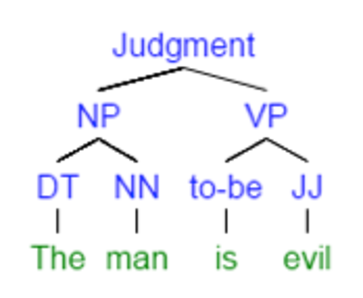
\includegraphics[width = .25\textwidth]{figs/judgment}
\caption{Example of Judgment Syntactic Parsing}
\label{fig:judgment}
\end{center}
\end{figure}

The number of flagged sentences divided by the total number of sentences was calculated for each document. This value was averaged for each document in the bin to generate the final judgment percentage signal.

\subsection{Context Vectors}
\label{sect:cv}

To capture the variations in linguistic flexibility of keywords within religious discourse, we implemented a context vector semantic density algorithm in python based on research by Sagi et al. 

Using the pre-processed tokens as described in the data section above, a co-occurrence matrix was constructed to capture how often each word appeared with other words in the vocabulary. This was done by iterating over each token in the bin and counting the words within +/- a \textit{k} sized window of the token. The result of this was a hashmap containing the full set of tokens with a count of the times each other token in the vocab occurred within a \textit{k}-sized window of it.  The values stored in this hashmap are condensed representations of the co-occurrence vectors, denoted as $V_i$, for each word \textit{i} over a vocabulary of length \textit{v} can be represented as such:

\begin{equation} 
\label{eq:context vector}
V_{i}=[x_{i1},x_{i2},...,x_{iv}]
\end{equation}
Where xiv is a word in the vocabulary that co-occurs with Vi.

Once the co-occurrence matrix was constructed, a distributional semantic matrix (DSM) was developed to reduce the computational load. The co-occurrence matrix was reduced to 100 components using truncated SVD. We opted to reduce our feature space to 100 components as it was the same value used in the work by \newcite{Sagi2009}. 

Following the development of the DSM, context vectors were created. The context vectors for each target word were developed by extracting the words within a \textit{k}-sized window surrounding the target word and summing the DSM vector for the words within the window.  As a result, the context $c_i$ represents information about the context in which a target term $w_i$ appears. For each of the \textit{l} occurrences of this target term, the context vector is defined as:

\begin{equation}
\label{eq:dsm}
c_{ij}=\sum_{k \epsilon window(w_{i})} dsm(w)
\end{equation}

To calculate the semantic density for each target word, we extracted the context vectors for that word. We then estimated the average cosine similarity of all the context vectors for that word by randomly sampling 2 context vectors from the set and calculating the cosine similarity between them. This was performed over \textit{n=1000} iterations. The resulting values were averaged; this was used to represent the semantic density for that target word.

\begin{equation}
\label{eq:semantic density}
semantic density(w) = \sum_{k=1}^{l-1} \frac{<c_{ik},c_{i(k+1)}>}{||c_{ik}||*||c_{i(k+1)}||}
\end{equation}

To determine the effect of the hyperparameters on average context vector cosine similarity, and in turn prediction, the co-occurrence window length and the context window length were varied. Discussion on the optimization of these parameters will be included in a later section.

\subsection{Network Quantification}
\label{sect:network}

Utilizing the DSM developed through the method described in the prior section, we created a graph to estimate semantic density using the igraph package in python \cite{Csardi2006}. We did this by assigning the words within a corpus as nodes and weighting the edges based on the cosine similarity of the word pairs. An algorithm was constructed to extract properties of this graph. First an adjacency matrix was defined by considering two nodes connected if they were below a threshold degree, which was varied in this analysis.  This graph was used to calculate eigenvector centrality.

Eigenvector centrality scores measure the influence of a network upon a node by looking at the number of influential nodes to which it is connected \cite{Estrada2005}. This was used as a proxy for the linguistic flexibility of a word, the more varied the connection the higher number of uses of that word.

\section{Hyperparameter Optimization}
\label{hyper}

To extend the previous work, key hyperparameters affecting the computation of the linguistic signals were identified. We believed that more effectively selecting and analyzing these variables would lead to a stronger prediction signal. Additionally, the assessment of the impact of these parameters could assist in extending this research to additional fields and discourse analyses.

\subsection{Co-occurrence Window}
\label{cooc window}

The first parameter selected for optimization was the co-occurrence window, $w_i$. This window directly affects the representation of the distribution of the language within the corpus. A larger window will incorporate more information about the words occurring around other words. This may better encapsulate the language or may add noise to the analysis. For this reason, windows of size 2 to 6 were explored during hyperparameter optimization. The ideal value was determined by that which best improved the accuracy of the model over a 3-fold cross validation.

\subsection{Context Window}
\label{sect:context window}

Context Window size was also analyzed to determine the optimal value. In contrast to the co-occurrence window which measures general word usage, the context window size impacts the specific measure of a word'��s usage. Without knowledge of how the proximity of a word affects the analysis of the variability of its usage, we sought to vary the window size from 2 to 6 to determine the window size with the best predictive performance.

\subsection{Network Adjacency Angle}
\label{sect:angle}

Finally, the parameter network adjacency angle threshold was optimized. As discussed in the signals section above, the network adjacency angle threshold was used to build connections between nodes in a graph. Nodes, representing words, whose cosine angle was below the angle, which in turn indicates similar word usage, were connected in the adjacency matrix. This graph was then used to calculate eigenvector centrality for each keyword. Any given threshold for connectivity between nodes could over or under estimate the relationship of words in the graph. Given the goal of accurately representing variability in word usage, the optimization of this parameter was  key factor. Once again the optimal threshold value was determined by varying the network angle by 15 degree increments over the range of 15 to 75 and selecting the parameter that most significantly improved model performance.


\section{Results}
\label{results}

In an effort to determine the effects of the hyperparameters on the semantic density and network signals, a grid search of the co-occurrence window, the context window and network adjacency angle was conducted. By varying these parameters we sought to better understand the effects of these parameters on the linguistic signals, but to also understand how these signals map to the linguistic rigidity of the sample groups. Through this understanding we hoped to in turn increase the prediction lift of the previously conducted analysis.

As shown in Figure \ref{fig:SD_surface} the average semantic density of the groups was mapped to the co-occurrence window and context vector window grid search. By plotting the average semantic density in relation to a co-occurrence window range of 2-6 and a context window range of 2-6, Figure \ref{fig:SD_surface} shows that an increase of these parameters results in an increase of the average semantic density of the keywords. These results are intuitive, as the increases of these parameters allows for greater information to be held in the context vectors, and in turn would result in a cosine similarity closer to one. The figure also shows that a limit is reached at a co-occurrence window of 5 and a context vector window of 5, where the average semantic density settles just above an average cosine similarity of 0.75. This indicates that little gain could be achieved by increasing these windows further, as there would be little distinction in the average semantic density of the keywords in the analysis.

\begin{figure}[!h]
\begin{center}
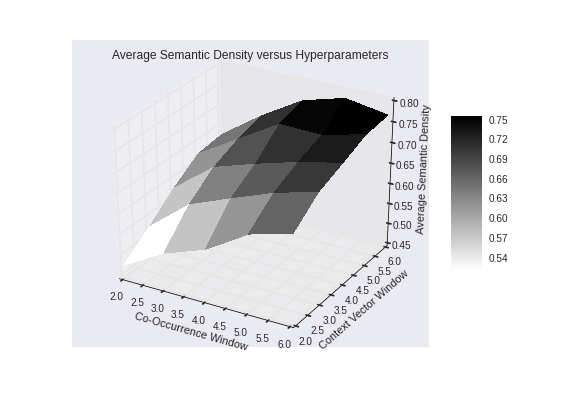
\includegraphics[width = .5\textwidth]{figs/SD_surface}
\caption{Average Semantic Density versus Hyperparameters}
\label{fig:SD_surface}
\end{center}
\end{figure}

To visualize the effects on the co-occurrence window size and network angle was plotted against the average eigenvector centrality. As seen in Figure \ref{fig:EVC_surface} the average eigenvector centrality trends upward as the co-occurrence window increases, and the network adjacency angle degrees. These results are also intuitive, as an increase in the co-occurrence window would result in a greater connection between the words within the discourse, and the lower adjacency angle would result in more edges between the nodes within the graphs. As eigenvector centrality is a bounded variable between 0 and 1, we see that the limit of 1 is nearly reached under the max conditions of 30 degrees and a co-occurrence window of 6, and we can hypothesize that this limit would be achieved upon increasing the co-occurrence window or decreasing the network angle further.

\begin{figure}[!h]
\begin{center}
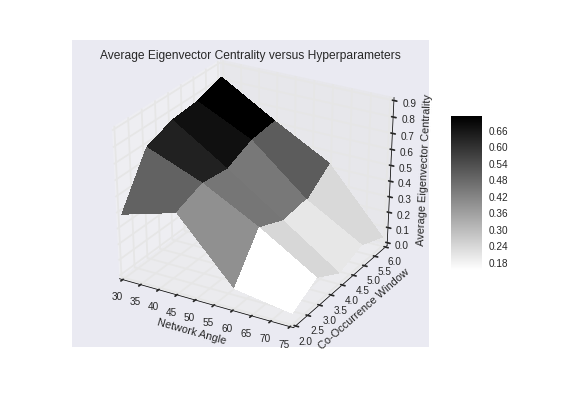
\includegraphics[width = .5\textwidth]{figs/EVC_surface}
\caption{Average Eigenvector Centrality versus Hyperparameters}
\label{fig:EVC_surface}
\end{center}
\end{figure}

In order to determine the relationship between average semantic density and group rank, the group rank was plotted against the average semantic density of the group, while varying the co-occurrence window and context vector. As seen in Figure \ref{fig:multipleAVGSD} the average semantic density is typically higher for groups with a lower rank, and the range between the highest semantic density and the lowest semantic density appears to decrease as the co-occurrence window and the context vector window increases. The ideal configuration of co-occurrence window and context vector window would yield a linear relationship between semantic density and group rank, as that would provided a linear separation boundary for the learning algorithms used. With this in mind a visual inspection of Figure \ref{fig:multipleAVGSD} indicates that a lower configuration may provide this trend, although there is not an explicit separation for any of the configurations.

\begin{figure}[!h]
\begin{center}
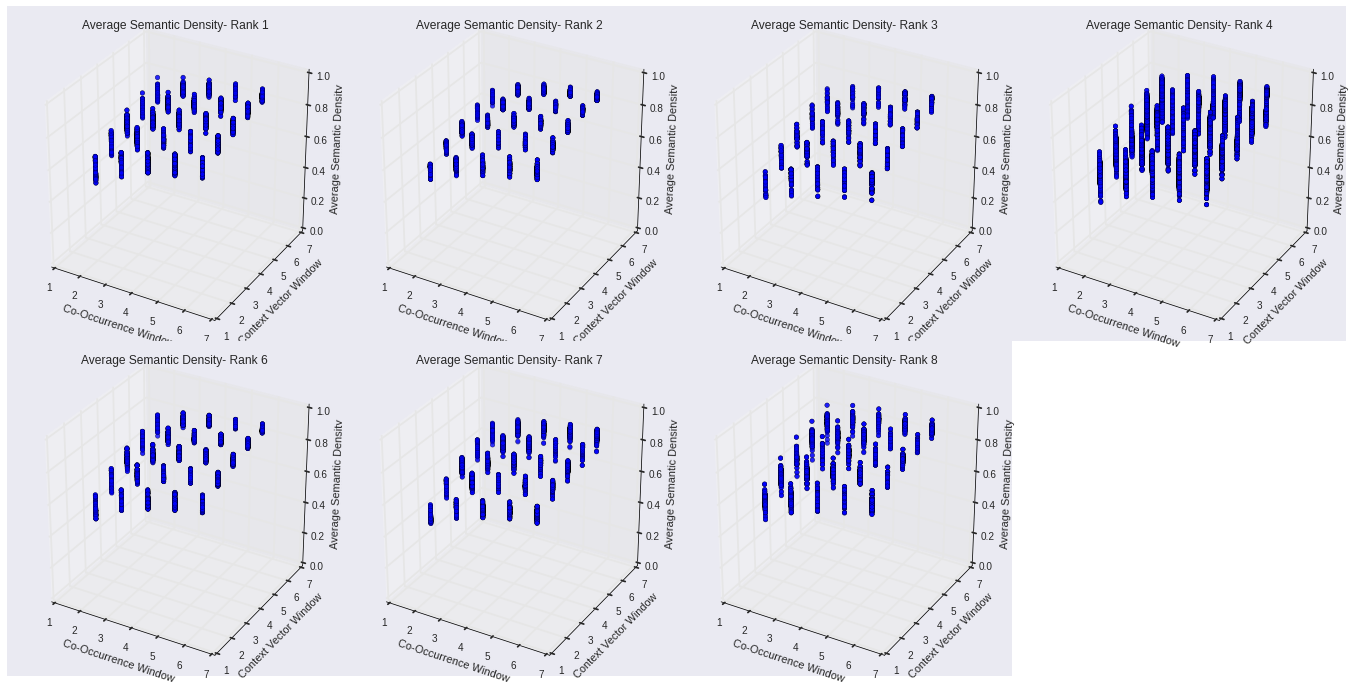
\includegraphics[width = \textwidth]{figs/multipleAVGSD}
\caption{Average Semantic Density versus Hyperparameters}
\label{fig:multipleAVGSD}
\end{center}
\end{figure}

Similar to the analysis above, we wanted to determine the distribution of average eigenvector centrality to group rank, as the co-occurrence window and network adjacency angle were varied. As depicted in Figure \ref{fig:multipleAVGEVC} the average eigenvector centrality distribution over group rank is disambiguous at minimum and maximum co-occurrence windows and network angles. Through visual inspection it appears that for none of the configurations there is a separable plane of average eigenvector centrality. As this metric is determined through the selection of keywords, it appears that a different methodology may need to be developed to identify influential keywords, rather than the one being utilized by the GRC-ERT.

\begin{figure}[!h]
\begin{center}
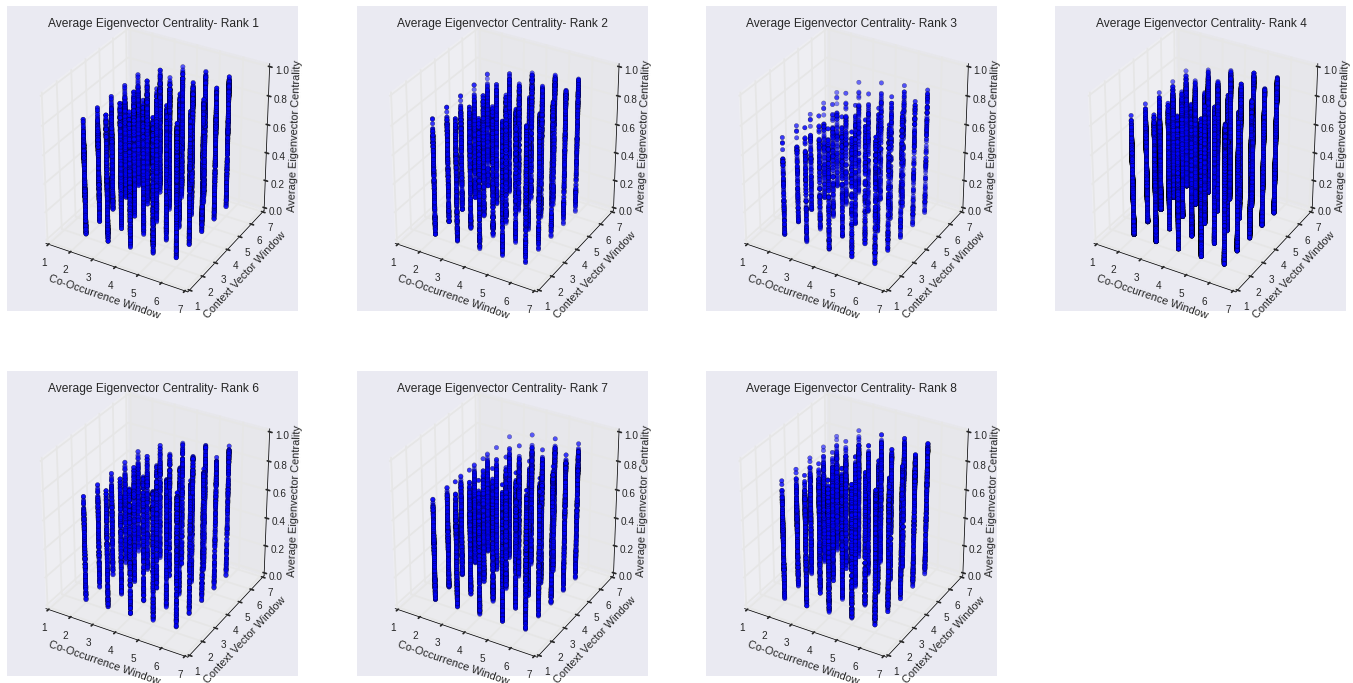
\includegraphics[width = \textwidth]{figs/multipleAVGEVC}
\caption{fig:multipleAVGEVC}
\label{fig:multipleAVGEVC}
\end{center}
\end{figure}

As seen in the previous analysis, we explored multiple modeling approaches to predict the linguistic rigidity of the religious sermons. In this analysis support vector machine regression (SVM-R) and random forest regression were used. These two models were selected because they are able to handle the bounded continuous response variable, as well as their ability to handle complex input relations. These models also outperformed the ANN and [] in the previous study.

We calculated model performance given an allowed error margin of 1, as shown in Eq. \ref{eq:acc 1} and Eq. \ref{eq:acc 2}, to account for the natural fluctuations in linguistic flexibility.

\begin{equation}
\label{eq:acc 1}
acc(bin, model) = 
\begin{cases} 
1, & \text{if } |\hat{y}-y| \leq 1 \\
0, & \text{otherwise}
\end{cases}
\end{equation}

\begin{equation}
\label{eq:acc 2}
acc(model) = \frac{1}{|bins|} \sum_{bin  \epsilon  bins} acc(bin, model)
\end{equation}

Using three-fold cross validation this mean absolute error (MAE) was utilized to determine the optimal hyper-parameter strategy for the two modeling approaches. MAE was chosen as the optimization parameter as it is not bounded as our accuracy metric is. Taking the medians of the accuracies and MAEs of the three-folds, Table \ref{table:TABLE_SVM} and Table \ref{table:TABLE_RF} provide the top five configurations for SVM-R and random forest, respectively.

\begin{table}[]
\centering
\caption{SVM}
\label{able:TABLE_SVM}
\begin{tabular}{|l|l|l|l|l|}
\hline
Co-Occurrence Window & Network Angle & Context Vector Window & Accuracy & MAE \\ \hline
5 & 6 & 30 & 85.85\% & 0.4464 \\ \hline
5 & 5 & 30 & 85.85\% & 0.449 \\ \hline
6 & 6 & 30 & 84.91\% & 0.451 \\ \hline
6 & 3 & 45 & 84.91\% & 0.4514 \\ \hline
6 & 6 & 45 & 84.91\% & 0.4519 \\ \hline
\end{tabular}
\end{table}

\begin{table}[]
\centering
\caption{Random Forest}
\label{table:TABLE_RF}
\begin{tabular}{|l|l|l|l|l|}
\hline
Co-Occurrence Window & Network Angle & Context Vector Window & Accuracy & MAE \\ \hline
2 & 75 & 2 & 92.45\% & 0.3085 \\ \hline
3 & 60 & 3 & 91.51\% & 0.3104 \\ \hline
3 & 60 & 2 & 90.57\% & 0.3123 \\ \hline
2 & 60 & 2 & 91.51\% & 0.3132 \\ \hline
3 & 75 & 2 & 91.51\% & 0.3170 \\ \hline
\end{tabular}
\end{table}

As seen above the greatest accuracy achieved by the random forest regression with a co-occurrence window of 2, a context vector window of 2 and a network angle of 75. With that said it is important to note that it is less computationally intensive to calculate lower angle network graphs, and smaller co-occurrence and context vector windows. With that in mind one may  consider to use the random forest configuration of a co-occurrence window of 2, and context vector window of 2 and a network angle of 60, as it would yield nearly identical prediction with less computational load. For the SVM-R the optimal configuration was a co-occurrence window of 5, a context vector window of 6 and a network angle of 30 degrees. Under these optimal conditions both the SVM-R and random forest regression outperformed the previous models whose prediction accuracies were 84\% and 86\%, respectively. It is important to note that due to the increase in data, and slight updates to the judgement and sentiment algorithms, it is difficult to perform a one to one comparison of the lift provided in this analysis. Under both these configurations, it appears that the random forest regression is the optimal model for this analysis, as it provides roughly a 6\% lift in accuracy.

\section{Conclusions}
\label{conclusions}

As the number of incidents of religious violence continues to increase, the need for scalable and accurate prediction systems intensifies. Analysis of the semantic characteristics of language has shown promise in prior research and the manual evaluation of performative characteristics by the GCR-ERT, has produced good predictions of flexibility of keywords in religious discourse. The work in this paper has significantly extended these previous results and shown the effects hyperparameter selection has on the performative features, and in turn the effects these parameters have on overall prediction accuracy. By visualizing these effects, a more informed methodology can be developed in future studies. 

While these results show promise, additional work is needed. As only a select set of values were tested due to computational demands of higher window sizes, further studies need to be conducted to further understand the effects of hyperparameters on these signals. Additionally, the process around identifying keywords needs to be further analyzed, so more robust group-specific keywords can be identified automatically, which may provide more separable trends in the network quantification and semantic density analyses. Lastly, a wider array of documents needs to be analyzed with a greater variety of religious groups in each class. This would prevent the algorithms from over-fitting based on group specific tendencies and illustrate the performative characteristics of these group'��s discourse.

\section*{Acknowledgements}

The acknowledgements should go immediately before the references.  Do
not number the acknowledgements section. Do not include this section
when submitting your paper for review.


\bibliographystyle{acl}
\bibliography{coling2016}

\end{document}
